\documentclass{extbook}[14pt]
\usepackage{multicol, enumerate, enumitem, hyperref, color, soul, setspace, parskip, fancyhdr, amssymb, amsthm, amsmath, bbm, latexsym, units, mathtools}
\everymath{\displaystyle}
\usepackage[headsep=0.5cm,headheight=0cm, left=1 in,right= 1 in,top= 1 in,bottom= 1 in]{geometry}
\usepackage{dashrule}  % Package to use the command below to create lines between items
\newcommand{\litem}[1]{\item #1

\rule{\textwidth}{0.4pt}}
\pagestyle{fancy}
\lhead{}
\chead{Answer Key for Makeup Progress Quiz 3 Version C}
\rhead{}
\lfoot{4315-3397}
\cfoot{}
\rfoot{Fall 2020}
\begin{document}
\textbf{This key should allow you to understand why you choose the option you did (beyond just getting a question right or wrong). \href{https://xronos.clas.ufl.edu/mac1105spring2020/courseDescriptionAndMisc/Exams/LearningFromResults}{More instructions on how to use this key can be found here}.}

\textbf{If you have a suggestion to make the keys better, \href{https://forms.gle/CZkbZmPbC9XALEE88}{please fill out the short survey here}.}

\textit{Note: This key is auto-generated and may contain issues and/or errors. The keys are reviewed after each exam to ensure grading is done accurately. If there are issues (like duplicate options), they are noted in the offline gradebook. The keys are a work-in-progress to give students as many resources to improve as possible.}

\rule{\textwidth}{0.4pt}

\begin{enumerate}\litem{
Construct the lowest-degree polynomial given the zeros below. Then, choose the intervals that contain the coefficients of the polynomial in the form $ax^3+bx^2+cx+d$.
\[ 6, \frac{2}{3}, \text{ and } \frac{-3}{5} \]

The solution is \( 15x^{3} -91 x^{2} + 36 \), which is option B.\begin{enumerate}[label=\Alph*.]
\item \( a \in [13, 17], b \in [87.9, 89.1], c \in [-13, -6], \text{ and } d \in [-42, -31] \)

$15x^{3} +89 x^{2} -12 x -36$, which corresponds to multiplying out $(x + 6)(3x -2)(5x + 3)$.
\item \( a \in [13, 17], b \in [-93.3, -90.6], c \in [-2, 4], \text{ and } d \in [35, 42] \)

* $15x^{3} -91 x^{2} + 36$, which is the correct option.
\item \( a \in [13, 17], b \in [89.6, 91.6], c \in [-2, 4], \text{ and } d \in [-42, -31] \)

$15x^{3} +91 x^{2} -36$, which corresponds to multiplying out $(x + 6)(3x + 2)(5x -3)$.
\item \( a \in [13, 17], b \in [106.9, 113.9], c \in [118, 124], \text{ and } d \in [35, 42] \)

$15x^{3} +109 x^{2} +120 x + 36$, which corresponds to multiplying out $(x + 6)(3x + 2)(5x + 3)$.
\item \( a \in [13, 17], b \in [-93.3, -90.6], c \in [-2, 4], \text{ and } d \in [-42, -31] \)

$15x^{3} -91 x^{2} -36$, which corresponds to multiplying everything correctly except the constant term.
\end{enumerate}

\textbf{General Comment:} To construct the lowest-degree polynomial, you want to multiply out $(x -6)(3x -2)(5x + 3)$
}
\litem{
Construct the lowest-degree polynomial given the zeros below. Then, choose the intervals that contain the coefficients of the polynomial in the form $x^3+bx^2+cx+d$.
\[ -5 + 2 i \text{ and } 3 \]

The solution is \( x^{3} +7 x^{2} -x -87 \), which is option C.\begin{enumerate}[label=\Alph*.]
\item \( b \in [-5, 4], c \in [-5.1, -3.5], \text{ and } d \in [4, 9] \)

$x^{3} + x^{2} -5 x + 6$, which corresponds to multiplying out $(x -2)(x -3)$.
\item \( b \in [-10, -3], c \in [-1.4, -0.2], \text{ and } d \in [84, 89] \)

$x^{3} -7 x^{2} -x + 87$, which corresponds to multiplying out $(x-(-5 + 2 i))(x-(-5 - 2 i))(x + 3)$.
\item \( b \in [4, 16], c \in [-1.4, -0.2], \text{ and } d \in [-90, -84] \)

* $x^{3} +7 x^{2} -x -87$, which is the correct option.
\item \( b \in [-5, 4], c \in [1, 2.4], \text{ and } d \in [-21, -11] \)

$x^{3} + x^{2} +2 x -15$, which corresponds to multiplying out $(x + 5)(x -3)$.
\item \( \text{None of the above.} \)

This corresponds to making an unanticipated error or not understanding how to use nonreal complex numbers to create the lowest-degree polynomial. If you chose this and are not sure what you did wrong, please contact the coordinator for help.
\end{enumerate}

\textbf{General Comment:} Remember that the conjugate of $a+bi$ is $a-bi$. Since these zeros always come in pairs, we need to multiply out $(x-(-5 + 2 i))(x-(-5 - 2 i))(x-(3))$.
}
\litem{
Construct the lowest-degree polynomial given the zeros below. Then, choose the intervals that contain the coefficients of the polynomial in the form $x^3+bx^2+cx+d$.
\[ 4 - 4 i \text{ and } -1 \]

The solution is \( x^{3} -7 x^{2} +24 x + 32 \), which is option D.\begin{enumerate}[label=\Alph*.]
\item \( b \in [1, 5], c \in [0, 10], \text{ and } d \in [0, 9] \)

$x^{3} + x^{2} +5 x + 4$, which corresponds to multiplying out $(x + 4)(x + 1)$.
\item \( b \in [1, 5], c \in [-10, 2], \text{ and } d \in [-10, 3] \)

$x^{3} + x^{2} -3 x -4$, which corresponds to multiplying out $(x -4)(x + 1)$.
\item \( b \in [5, 9], c \in [17, 29], \text{ and } d \in [-32, -27] \)

$x^{3} +7 x^{2} +24 x -32$, which corresponds to multiplying out $(x-(4 - 4 i))(x-(4 + 4 i))(x -1)$.
\item \( b \in [-12, -3], c \in [17, 29], \text{ and } d \in [32, 35] \)

* $x^{3} -7 x^{2} +24 x + 32$, which is the correct option.
\item \( \text{None of the above.} \)

This corresponds to making an unanticipated error or not understanding how to use nonreal complex numbers to create the lowest-degree polynomial. If you chose this and are not sure what you did wrong, please contact the coordinator for help.
\end{enumerate}

\textbf{General Comment:} Remember that the conjugate of $a+bi$ is $a-bi$. Since these zeros always come in pairs, we need to multiply out $(x-(4 - 4 i))(x-(4 + 4 i))(x-(-1))$.
}
\litem{
Construct the lowest-degree polynomial given the zeros below. Then, choose the intervals that contain the coefficients of the polynomial in the form $ax^3+bx^2+cx+d$.
\[ \frac{7}{4}, \frac{7}{3}, \text{ and } -1 \]

The solution is \( 12x^{3} -37 x^{2} + 49 \), which is option D.\begin{enumerate}[label=\Alph*.]
\item \( a \in [5, 19], b \in [-39, -36], c \in [-4, 2], \text{ and } d \in [-52, -46] \)

$12x^{3} -37 x^{2} -49$, which corresponds to multiplying everything correctly except the constant term.
\item \( a \in [5, 19], b \in [56, 69], c \in [95, 101], \text{ and } d \in [47, 55] \)

$12x^{3} +61 x^{2} +98 x + 49$, which corresponds to multiplying out $(4x + 7)(3x + 7)(x + 1)$.
\item \( a \in [5, 19], b \in [2, 7], c \in [-61, -52], \text{ and } d \in [-52, -46] \)

$12x^{3} +5 x^{2} -56 x -49$, which corresponds to multiplying out $(4x + 7)(3x -7)(x + 1)$.
\item \( a \in [5, 19], b \in [-39, -36], c \in [-4, 2], \text{ and } d \in [47, 55] \)

* $12x^{3} -37 x^{2} + 49$, which is the correct option.
\item \( a \in [5, 19], b \in [36, 41], c \in [-4, 2], \text{ and } d \in [-52, -46] \)

$12x^{3} +37 x^{2} -49$, which corresponds to multiplying out $(4x + 7)(3x + 7)(x -1)$.
\end{enumerate}

\textbf{General Comment:} To construct the lowest-degree polynomial, you want to multiply out $(4x -7)(3x -7)(x + 1)$
}
\litem{
Describe the zero behavior of the zero $x = 4$ of the polynomial below.
\[ f(x) = -5(x - 4)^{4}(x + 4)^{9}(x - 2)^{3}(x + 2)^{7} \]

The solution is the graph below, which is option B.
\begin{center}
    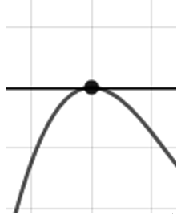
\includegraphics[width=0.3\textwidth]{../Figures/polyZeroBehaviorBC.png}
\end{center}\begin{enumerate}[label=\Alph*.]
\begin{multicols}{2}
\item 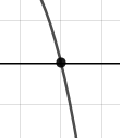
\includegraphics[width = 0.3\textwidth]{../Figures/polyZeroBehaviorAC.png}
\item 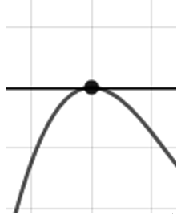
\includegraphics[width = 0.3\textwidth]{../Figures/polyZeroBehaviorBC.png}
\item 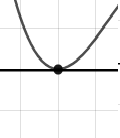
\includegraphics[width = 0.3\textwidth]{../Figures/polyZeroBehaviorCC.png}
\item 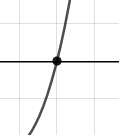
\includegraphics[width = 0.3\textwidth]{../Figures/polyZeroBehaviorDC.png}
\end{multicols}\item None of the above.\end{enumerate}
\textbf{General Comment:} You will need to sketch the entire graph, then zoom in on the zero the question asks about.
}
\litem{
Which of the following equations \textit{could} be of the graph presented below?

\begin{center}
    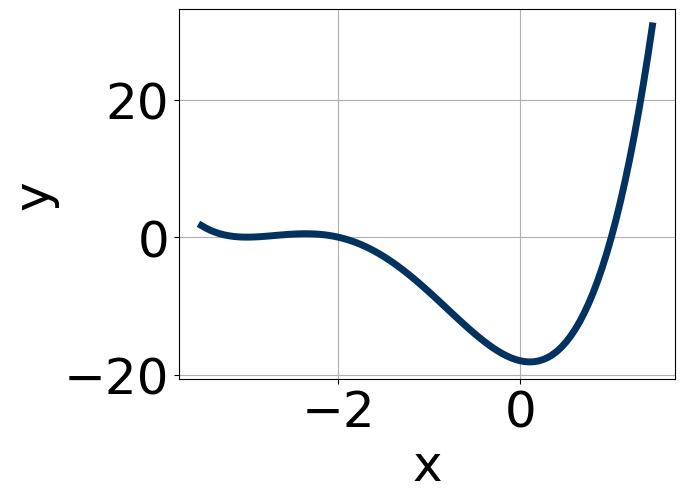
\includegraphics[width=0.5\textwidth]{../Figures/polyGraphToFunctionCopyC.png}
\end{center}




The solution is \( 8(x + 3)^{4} (x + 2)^{5} (x - 1)^{9} \), which is option B.\begin{enumerate}[label=\Alph*.]
\item \( 17(x + 3)^{9} (x + 2)^{4} (x - 1)^{9} \)

The factor $-3$ should have an even power and the factor $-2$ should have an odd power.
\item \( 8(x + 3)^{4} (x + 2)^{5} (x - 1)^{9} \)

* This is the correct option.
\item \( 11(x + 3)^{10} (x + 2)^{10} (x - 1)^{7} \)

The factor $(x + 2)$ should have an odd power.
\item \( -3(x + 3)^{8} (x + 2)^{5} (x - 1)^{9} \)

This corresponds to the leading coefficient being the opposite value than it should be.
\item \( -3(x + 3)^{4} (x + 2)^{9} (x - 1)^{8} \)

The factor $(x - 1)$ should have an odd power and the leading coefficient should be the opposite sign.
\end{enumerate}

\textbf{General Comment:} General Comments: Draw the x-axis to determine which zeros are touching (and so have even multiplicity) or cross (and have odd multiplicity).
}
\litem{
Describe the zero behavior of the zero $x = 6$ of the polynomial below.
\[ f(x) = 5(x + 3)^{8}(x - 3)^{4}(x - 6)^{13}(x + 6)^{8} \]

The solution is the graph below, which is option D.
\begin{center}
    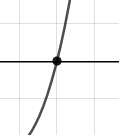
\includegraphics[width=0.3\textwidth]{../Figures/polyZeroBehaviorCopyDC.png}
\end{center}\begin{enumerate}[label=\Alph*.]
\begin{multicols}{2}
\item 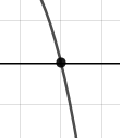
\includegraphics[width = 0.3\textwidth]{../Figures/polyZeroBehaviorCopyAC.png}
\item 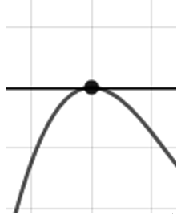
\includegraphics[width = 0.3\textwidth]{../Figures/polyZeroBehaviorCopyBC.png}
\item 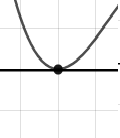
\includegraphics[width = 0.3\textwidth]{../Figures/polyZeroBehaviorCopyCC.png}
\item 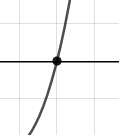
\includegraphics[width = 0.3\textwidth]{../Figures/polyZeroBehaviorCopyDC.png}
\end{multicols}\item None of the above.\end{enumerate}
\textbf{General Comment:} You will need to sketch the entire graph, then zoom in on the zero the question asks about.
}
\litem{
Which of the following equations \textit{could} be of the graph presented below?

\begin{center}
    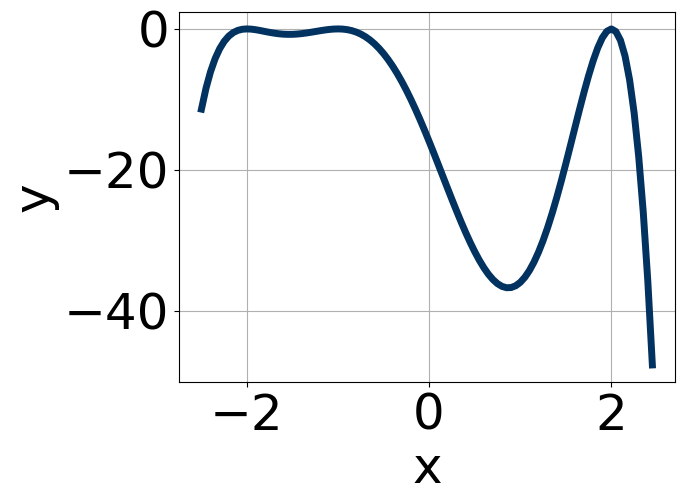
\includegraphics[width=0.5\textwidth]{../Figures/polyGraphToFunctionC.png}
\end{center}




The solution is \( -19(x - 2)^{8} (x + 2)^{4} (x + 1)^{4} \), which is option D.\begin{enumerate}[label=\Alph*.]
\item \( 7(x - 2)^{4} (x + 2)^{6} (x + 1)^{9} \)

The factor $(x + 1)$ should have an even power and the leading coefficient should be the opposite sign.
\item \( -4(x - 2)^{8} (x + 2)^{11} (x + 1)^{9} \)

The factors $(x + 2)$ and $(x + 1)$ should both have even powers.
\item \( 13(x - 2)^{4} (x + 2)^{8} (x + 1)^{6} \)

This corresponds to the leading coefficient being the opposite value than it should be.
\item \( -19(x - 2)^{8} (x + 2)^{4} (x + 1)^{4} \)

* This is the correct option.
\item \( -16(x - 2)^{6} (x + 2)^{4} (x + 1)^{11} \)

The factor $(x + 1)$ should have an even power.
\end{enumerate}

\textbf{General Comment:} General Comments: Draw the x-axis to determine which zeros are touching (and so have even multiplicity) or cross (and have odd multiplicity).
}
\litem{
Describe the end behavior of the polynomial below.
\[ f(x) = 4(x + 5)^{5}(x - 5)^{10}(x - 2)^{3}(x + 2)^{5} \]

The solution is the graph below, which is option D.
\begin{center}
    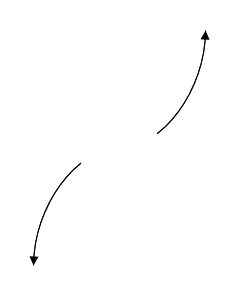
\includegraphics[width=0.3\textwidth]{../Figures/polyEndBehaviorCopyDC.png}
\end{center}\begin{enumerate}[label=\Alph*.]
\begin{multicols}{2}
\item 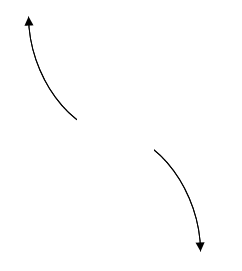
\includegraphics[width = 0.3\textwidth]{../Figures/polyEndBehaviorCopyAC.png}
\item 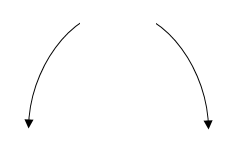
\includegraphics[width = 0.3\textwidth]{../Figures/polyEndBehaviorCopyBC.png}
\item 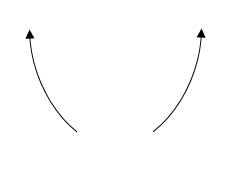
\includegraphics[width = 0.3\textwidth]{../Figures/polyEndBehaviorCopyCC.png}
\item 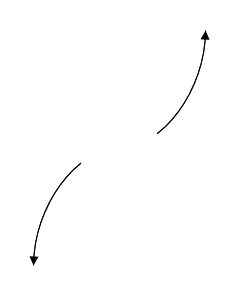
\includegraphics[width = 0.3\textwidth]{../Figures/polyEndBehaviorCopyDC.png}
\end{multicols}\item None of the above.\end{enumerate}
\textbf{General Comment:} Remember that end behavior is determined by the leading coefficient AND whether the \textbf{sum} of the multiplicities is positive or negative.
}
\litem{
Describe the end behavior of the polynomial below.
\[ f(x) = 4(x + 6)^{2}(x - 6)^{5}(x + 4)^{2}(x - 4)^{2} \]

The solution is the graph below, which is option D.
\begin{center}
    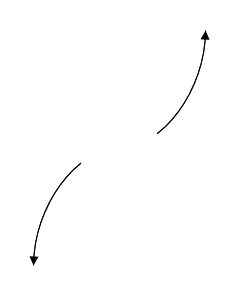
\includegraphics[width=0.3\textwidth]{../Figures/polyEndBehaviorDC.png}
\end{center}\begin{enumerate}[label=\Alph*.]
\begin{multicols}{2}
\item 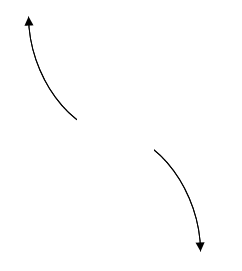
\includegraphics[width = 0.3\textwidth]{../Figures/polyEndBehaviorAC.png}
\item 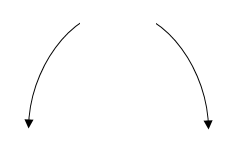
\includegraphics[width = 0.3\textwidth]{../Figures/polyEndBehaviorBC.png}
\item 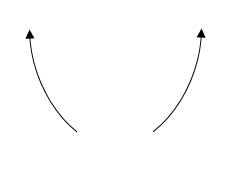
\includegraphics[width = 0.3\textwidth]{../Figures/polyEndBehaviorCC.png}
\item 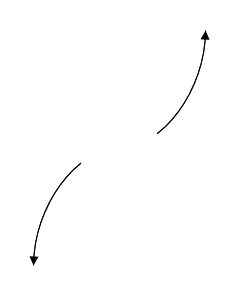
\includegraphics[width = 0.3\textwidth]{../Figures/polyEndBehaviorDC.png}
\end{multicols}\item None of the above.\end{enumerate}
\textbf{General Comment:} Remember that end behavior is determined by the leading coefficient AND whether the \textbf{sum} of the multiplicities is positive or negative.
}
\end{enumerate}

\end{document}